\section{}

\subsection{}
\textbf{A Pb–$60$ at\% Sn alloy was slowly cooled from $380^{\circ}$C to $50^{\circ}$C. Calculate the volume fraction of the primary phase at $50^{\circ}$C.}

The phase diagram for an alloy of Pb and Sn is shown in figure \ref{fig:diagrama}. The temperature and composition are located in the diagram, the composition $C_0$ corresponds to a $60$\% of Sn and $40$\% of Pb. From the figure, it can be seen that for a temperature of $50^{\circ}$C there is presence of two phases, $\alpha$ and $\beta$. From the isothermal of the temperature it is possible to obtain the values of the compositions for each phase by intersecting the ishothermal llinea with the baoundaries of the phase diagram, which gives the following results:

\begin{align}
    \label{eq:compostitions}
    \begin{split}
        C_{Sn_{\alpha}}&=4\% \\ C_{Sn_{\beta}}&=99\% \\ C_{Pb_{\alpha}}&=96\% \\ C_{Pb_{\beta}}&=1\%,
    \end{split}
\end{align}
where $C_{Sn_{\alpha}}$ is the composition of Sn in the $\alpha$ phase, $C_{Sn_{\beta}}$ is the composition of Sn in the $\beta$ phase, $C_{Pb_{\alpha}}$ the composition of Pb in the $\alpha$ phase and, $C_{Pb_{\beta}}$ is the composition of Pb in the $\beta$ phase.

The primary phase is the phase that has a higher fraction in the mixture, for which is necessary to calcualte the fraction of each phase, and to do that the lever rule is used. The lever rule states that the phase fraction can be calculated taking the distance of the tie line of the total composition to the border of the other phase and divide this by the total distance of the tie line, the expressions for the mass fractions are presented in the following equations:

\begin{align}
    \label{eq:frac_alpha}
    W_{\alpha}&=\dfrac{C_{\beta}-C_0}{C_{\beta}-C_{\alpha}}
\end{align}
and
\begin{align}
    \label{eq:frac_beta}
    W_{\beta}&=\dfrac{C_0-C_{\alpha}}{C_{\beta}-C_{\alpha}};
\end{align}
where $W_{\alpha}$ is the fraction of the $\alpha$ phase, $W_{\beta}$ is the fraction of the $\beta$ phase, $C_{\alpha}$ and $C_{\beta}$ are the compositions of the $\alpha$ and $\beta$ phases, and $C_0$ is the initial composition \citep[p.~290-291]{callister2010materials}. 

\begin{figure}[h]
    \centering
    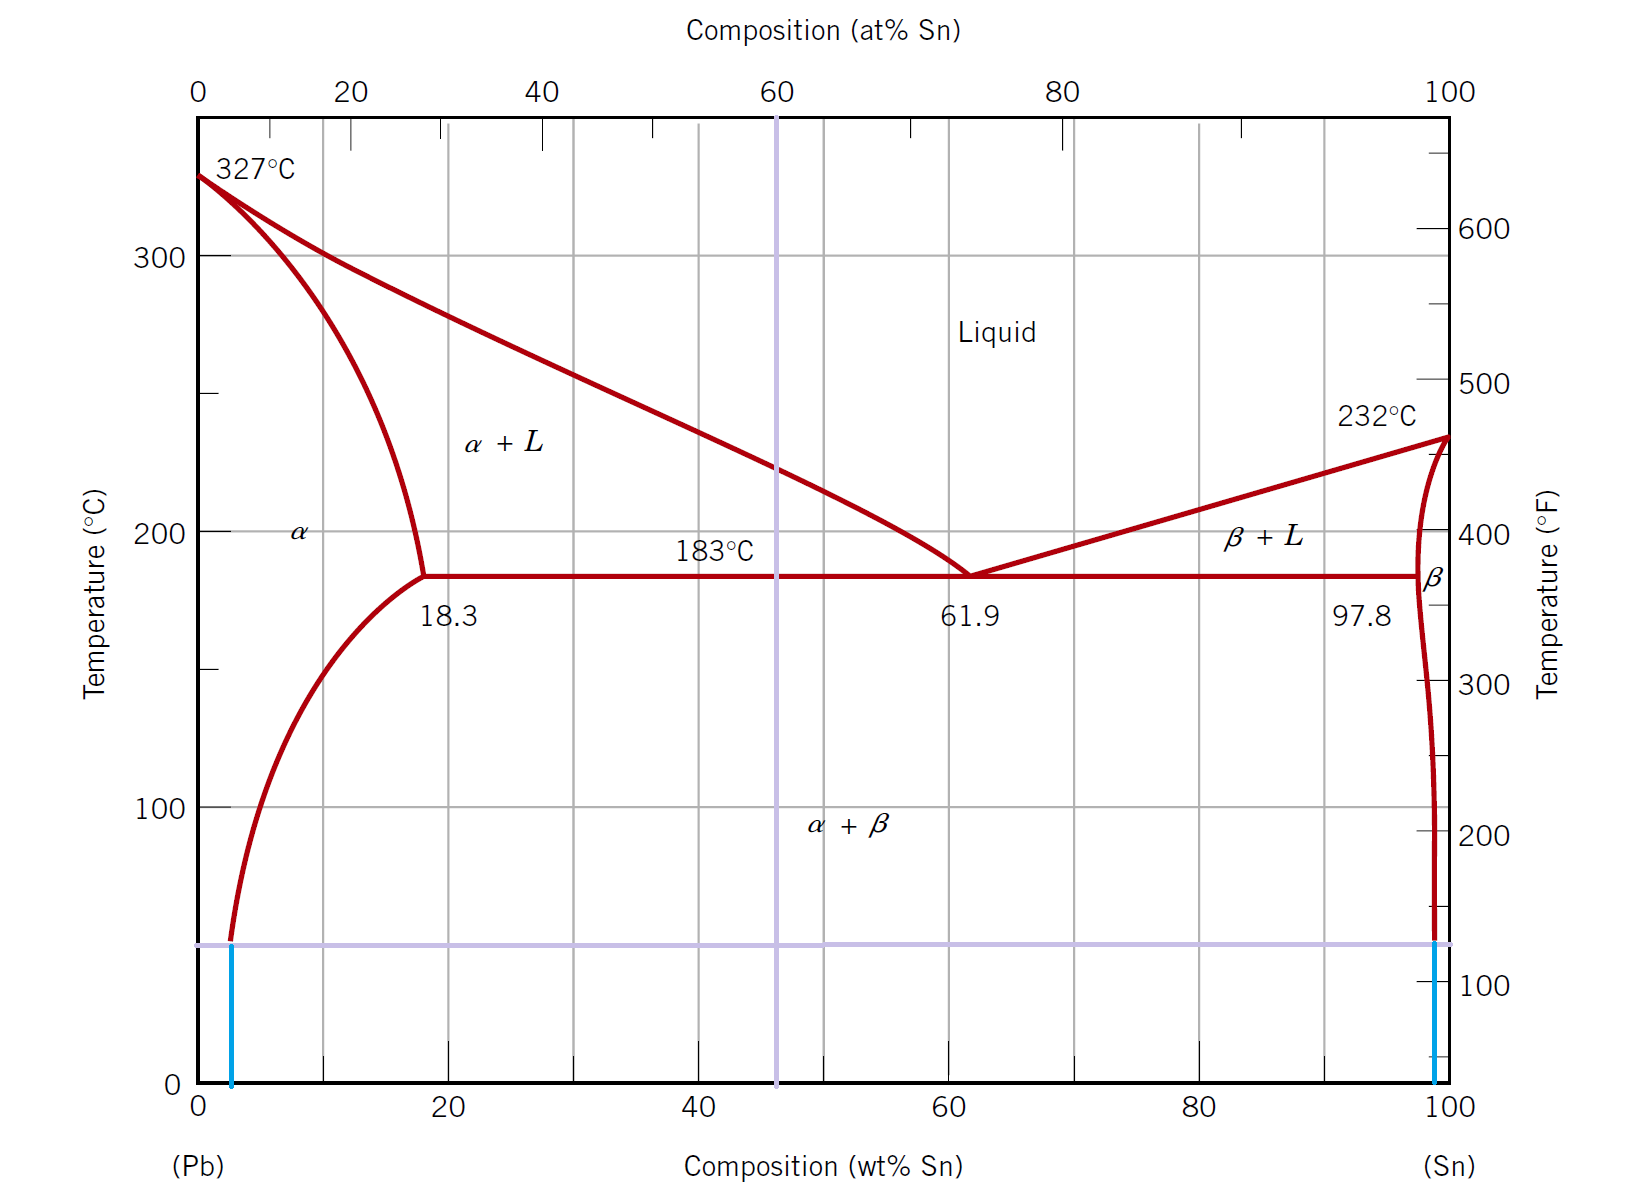
\includegraphics[width=0.93\textwidth]{graficas/diagrama.png}
    \caption{Phase diagram for lead-tin \\
    \textit{Source: Figure adapted from \citep{callister2010materials}}}
    \label{fig:diagrama}
\end{figure}

Using the values of the compositions for Sn from equation \ref{eq:compostitions} obtained from the phase diagram in figure \ref{fig:diagrama}, the fractions for $\alpha$ and $\beta$ phases are calculated using equations \eqref{eq:frac_alpha} and \eqref{eq:frac_beta}:

\begin{align}
    \label{eq:w_alpha}
    W_{\alpha}&=\dfrac{C_{\beta}-C_0}{C_{\beta}-C_{\alpha}} =\dfrac{99-60}{99-4} = \dfrac{39}{95} = 0.410526
\end{align}

\begin{align}
    \label{eq:w_beta}
    W_{\beta}&=\dfrac{C_0-C_{\alpha}}{C_{\beta}-C_{\alpha}} =\dfrac{60-4}{99-4} =\dfrac{59}{95} =0.589474
\end{align}

Based on the results obtained, it can be determined that the primary phase, the one that has a higher fraction, is the $\beta$ phase. The equation for the volumen fraction for the $\beta$ phase is given by:

\begin{align}
    \label{eq:vol_beta}
    V_{\beta}&=\dfrac{\dfrac{W_{\beta}}{\rho_{\beta}}}{\dfrac{W_{\alpha}}{\rho_{\alpha}}+\dfrac{W_{\beta}}{\rho_{\beta}}},
\end{align}
where $V_{\beta}$ is the volumen fraction of the $\beta$ phase, $W_{\alpha}$ and $W_{\beta}$ are the fractions of both $\alpha$ and $\beta$ phases, and $\rho_{alpha}$ and $\rho_{\beta}$ are the densities of $\alpha$ and $\beta$ phases respectively \citep[p.~293]{callister2010materials}.

From equation \eqref{eq:vol_beta} it can be seen that it is necessary to calculate the density of each phase, which can be done by using the following equations:

\begin{align}
    \label{eq:rho_alpha}
    \rho_{\alpha}&=\dfrac{100}{\dfrac{C_{Sn_{\alpha}}}{\rho_{Sn}}+\dfrac{C_{Pb_{\alpha}}}{\rho_{Pb}}}
\end{align}
and
\begin{align}
    \label{eq:rho_beta}
    \rho_{\beta}&=\dfrac{100}{\dfrac{C_{Sn_{\beta}}}{\rho_{Sn}}+\dfrac{C_{Pb_{\beta}}}{\rho_{Pb}}},
\end{align}
where $\rho_{\alpha}$ and $\rho_{\beta}$ are the densities for each phase, $C_{Sn_{\alpha}}$ and $C_{Pb_{\alpha}}$ are the compositions of Sn and Pb in the $\alpha$ phase, $C_{Sn_{\beta}}$ and $C_{Pb_{\beta}}$ are the compositions of Sn and Pb in the $\beta$ phase, and $\rho_{Sn}$ and $\rho_{Pb}$ are the densities for Sn and Pb \citep[p.~97]{callister2010materials}.

Using equations \eqref{eq:rho_alpha} and \eqref{eq:rho_beta}, with the values for the densities: $\rho_{Sn}=7.24$ and $\rho_{Pb}=11.23$ (g/cm$^3$) \citep{callister2010materials} as well as the composition of the phases obtained from the phase diagrams from equation \ref{eq:compostitions}, the densities for each phases are obtained:
\shnote{me quede editando aca}

\begin{align}
    \label{eq:rho_alpha_num}
    \rho_{\alpha}&=\dfrac{100}{\dfrac{4}{7.24}+\dfrac{96}{11.23}}=10.987783
\end{align}

\begin{align}
    \label{eq:rho_beta_num}
    \rho_{\beta}&=\dfrac{100}{\dfrac{99}{7.24}+\dfrac{1}{11.23}}=7.265815
\end{align}

From the values of the density of each phase and the fraction of the phases, the volume fraction can be calculated using equation \eqref{eq:vol_beta}:

\begin{align}
    \label{eq:vol_beta_num}
    V_{\beta}&=\dfrac{\dfrac{W_{\beta}}{\rho_{\beta}}}{\dfrac{W_{\alpha}}{\rho_{\alpha}}+\dfrac{W_{\beta}}{\rho_{\beta}}}=\dfrac{\dfrac{0.589474}{7.265815}}{\dfrac{0.410526}{10.987783}+\dfrac{0.589474}{7.265815}}=0.684686\eqsim 0.68
\end{align}

%\begin{figure}[h]
%    \centering
%    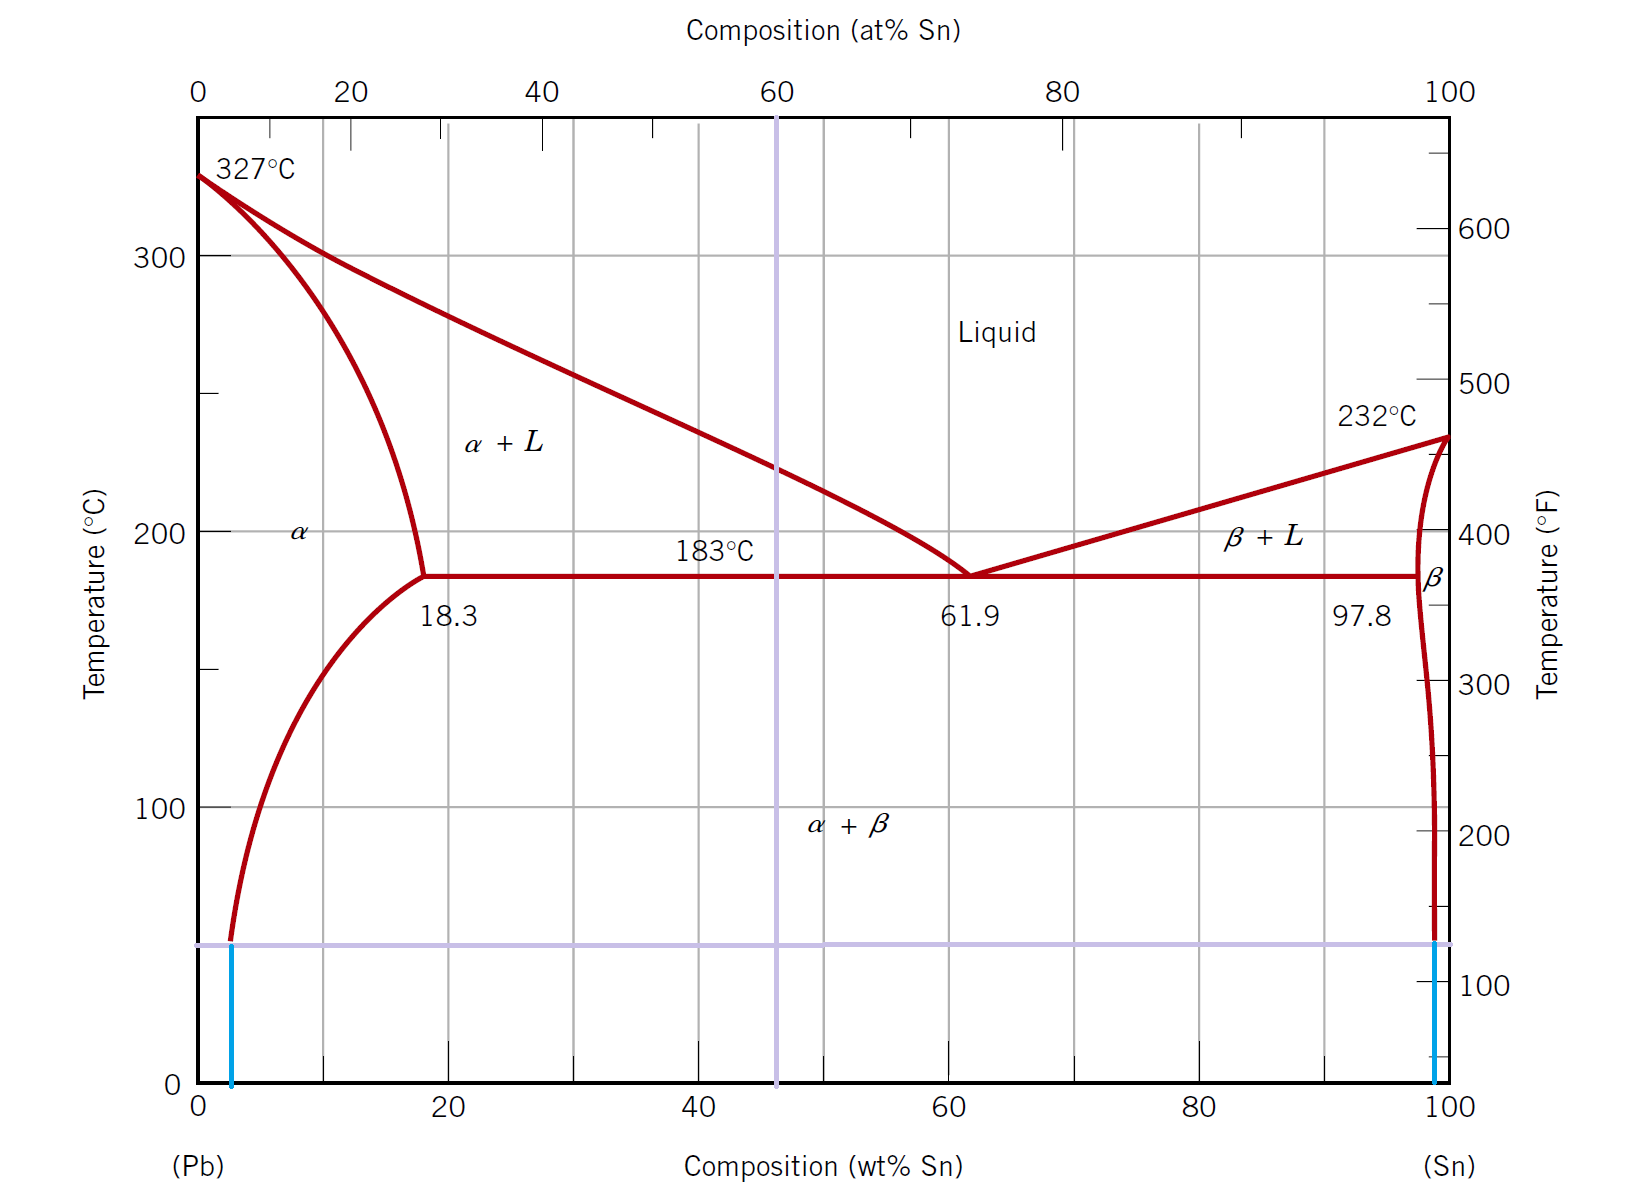
\includegraphics[width=1\textwidth]{graficas/diagrama.png}
%    \caption{Phase diagram for lead-tin \\
%    \textit{Source: Figure adapted from \citep{callister2010materials}}}
%    \label{fig:diagrama}
%\end{figure}

\begin{mdframed}
The volumen fraction of the primary phase is 0.68.
\end{mdframed}

\newpage
\subsection{}
A Pb–$25$ at$\%$ Sn alloy was slowly cooled from 380°C to 50°C. Ideally, Sn phase is expected to precipitate within Pb-phase grains, but in reality, a eutectic structure appeared. Assuming there were no experimental issues such as weighing errors, discuss the reason why this phenomenon occurred.

%\begin{mdframed}
\shnote{Aca creo que deberia de ir la discusion del punto eutectico, pero ahorita no me acuerdo por que es que se forma esa cosa :c}
%\end{mdframed}